% concatenated from visibility_improvement.tex
\documentclass[11pt,a4paper]{amsart}
\usepackage[margin=1in]{geometry}
\usepackage[T1]{fontenc}
\usepackage{amsmath,amssymb,amsthm}
\usepackage{tikz}
\usetikzlibrary{arrows.meta}
\usepackage[hidelinks]{hyperref}
\newtheorem{theorem}{Theorem}
\newtheorem{lemma}[theorem]{Lemma}
\title{Four collinear points or six visible points}
\author{Stijn Cambie}
\thanks{Department of Computer Science, KU Leuven Campus Kulak-Kortrijk, 8500 Kortrijk, Belgium. Supported by a postdoctoral fellowship from the Research Foundation Flanders (FWO), grant number 1225224N}
\date{}
\hypersetup{pdftitle={Four collinear points or six visible points},
pdfsubject={A short proof that N(4,6) is at most 880}}
\begin{document}
\pagestyle{plain}
\begin{abstract}
Every finite planar set of at least $880$ points contains four collinear
points or six pairwise visible points. 
% An elementary graph estimate and
% two convex partitions give a short proof.
\end{abstract}
\maketitle
\section{Introduction}

Let $P$ be a finite set of points in the plane. Two distinct points of $P$
are \emph{visible} if the open segment joining them contains no point of
$P$. The \emph{visibility graph} $G(P)$ has vertex set $P$ and an edge
for each visible pair. A point on the open segment joining a nonvisible
pair is called a \emph{blocker} of that pair.
For integers $s,t\ge3$, let $N(s,t)$ be the least integer, if it exists,
such that every finite planar set of at least $N(s,t)$ points contains
$s$ collinear points or $t$ pairwise visible points.

K\'ara, P\'or, and Wood~\cite{KPW} introduced the
\emph{big-line--big-clique conjecture} in 2005: $N(s,t)$ is finite for
every fixed $s,t$. The case $N(3,t)=t$ is immediate, since without three
collinear points every pair is visible. Also $N(s,3)=s$: every
noncollinear finite set contains a triangle of minimum positive area,
whose vertices are pairwise visible.
K\'ara, P\'or, and Wood proved finiteness for $t\le4$.
Abel et al.~\cite{ABBCetal} established the case $t=5$ for every $s$,
and Bar\'at et al.~\cite{Barat} later obtained the quadratic bound
$N(s,5)\le328s^2$ through their theorem on empty pentagons.
In 2026, Bonnet~\cite{Bonnet} proved $N(4,6)\le10^{11055931}$,
settling the next open case. We give a short proof that
\[
                         N(4,6)\le880.
\]

A related, weaker question replaces the clique number by the chromatic
number: for fixed $s\ge3$ and $c\ge2$, is the size of $P$ bounded if $P$ has no
$s$ collinear points and $G(P)$ can be properly colored with $c$ colors?
This would follow from $N(s,c+1)<\infty$, since a $c$-colorable graph
contains no $K_{c+1}$. Hujter and Kisfaludi-Bak~\cite{HKB} proved this
chromatic version for $s=4$ and $c=5$, giving an upper bound of $2310$
points. More precisely, their Theorem~15 gives $5h(6)-5$, where $h(6)$
is the least number of points in general position that forces an empty
convex hexagon. Here \emph{general position} means that no three points
are collinear, and \emph{empty} means that the convex hull contains no
other point of the set.
Heule and Scheucher's computer-assisted theorem~\cite{HS} gives
$h(6)=30$. Thus we use the following consequence:
\begin{quote}
A finite planar set with no four collinear points and a $5$-colorable
visibility graph has at most $145$ points.
\end{quote}
The proof, presented in the next section, is elementary (the bound can be improved by extending the computations, but we have no guess about the exact value).

\section{Proof}

For a graph $H$, write $e(H)$ for its number of edges and $N_H(v)$ for
the set of neighbors of a vertex $v$.


\begin{lemma}\label{graph}
If a $K_6$-free graph $H$ on $r\ge1$ vertices requires at least $q$ vertex deletions
to become $5$-colorable, where $0\le q\le r$, then
\[
             e(H)\le\frac{2r^2}{5}-\frac{q(r-q)}{10}.
\]
\end{lemma}
\begin{proof}
We start building a maximal clique vertex by vertex. Set $R_1=V(H)$.
For each $i$ with $R_i\ne\varnothing$, choose $v_i\in R_i$ of largest
degree in the original graph $H$, and put
$R_{i+1}=R_i\cap N_H(v_i)$.
Stop when $R_{k+1}=\varnothing$. Each chosen vertex is adjacent to all
earlier choices, and the stopping condition makes
$\{v_1,\ldots,v_k\}$ a maximal clique; see Figure~\ref{greedy}
(cf.~\cite[Section~2]{BN}).

Put $A_i=R_i\setminus R_{i+1}$. Thus $A_i$ consists of the vertices
whose first nonneighbor in the sequence is $v_i$, counting $v_i$ itself
as a nonneighbor. The sets $A_i$ partition $V(H)$.
Let $a_i=|A_i|$, $d_i=d_H(v_i)$, and
$\varepsilon_i=r-a_i-d_i\ge0$.
Each vertex of $A_i$ was available when $v_i$ was chosen, so
\[
       2e(H)\le\sum_i a_i d_i
       =r^2-\sum_i(a_i^2+a_i\varepsilon_i).
\]
If $k\le4$, Cauchy's inequality gives $e(H)\le3r^2/8$, which suffices
since $q(r-q)\le r^2/4$. Thus assume $k=5$.
Deleting the vertices missing two or more clique vertices leaves five
independent sets: an edge between two vertices missing only $v_i$ would
complete a $K_6$ with the other four clique vertices. Since
$\sum_i\varepsilon_i$ counts all misses beyond the first, it is at least
$q$. Choose $0\le x_i\le\varepsilon_i$ with $\sum_i x_i=q$. Then by Cauchy-Schwarz again
\[
 \sum_i(a_i^2+a_i\varepsilon_i)
 \ge\sum_i(a_i+x_i/2)^2-\frac14\sum_i x_i^2
 \ge\frac{(r+q/2)^2}{5}-\frac{q^2}{4}
 =\frac{r^2+q(r-q)}5.
\]
\end{proof}

\begin{figure}[htbp]
\centering
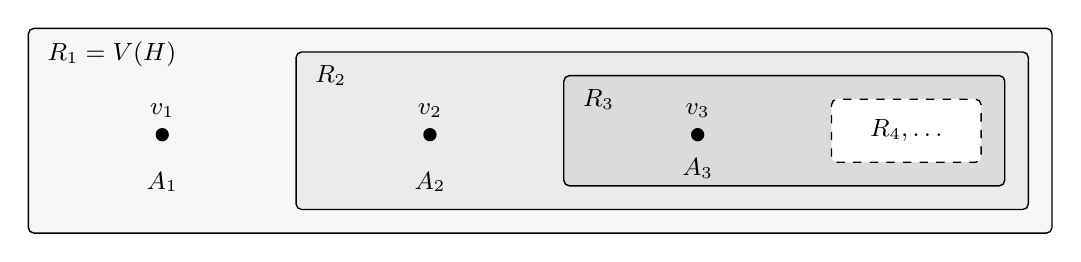
\begin{tikzpicture}[x=1cm,y=1cm,font=\small,
  region/.style={draw,rounded corners=2pt,line width=.5pt},
  point/.style={circle,fill=black,inner sep=1.7pt}]
  \path[region,fill=black!3] (0,0) rectangle (13,2.6);
  \path[region,fill=black!8] (3.4,.3) rectangle (12.7,2.3);
  \path[region,fill=black!14] (6.8,.6) rectangle (12.4,2.0);
  \path[region,dashed,fill=white] (10.2,.9) rectangle (12.1,1.7);
  \node[anchor=north west] at (.12,2.55) {$R_1=V(H)$};
  \node[anchor=north west] at (3.52,2.25) {$R_2$};
  \node[anchor=north west] at (6.92,1.95) {$R_3$};
  \node at (11.15,1.3) {$R_4,\ldots$};
  \node[point,label=above:$v_1$] at (1.7,1.25) {};
  \node[point,label=above:$v_2$] at (5.1,1.25) {};
  \node[point,label=above:$v_3$] at (8.5,1.25) {};
  \node at (1.7,.65) {$A_1$};
  \node at (5.1,.65) {$A_2$};
  \node at (8.5,.82) {$A_3$};
  % \draw[-{Stealth[length=4pt]}] (1.7,-.42) --
  %   node[below] {$\cap N_H(v_1)$} (5.1,-.42);
  % \draw[-{Stealth[length=4pt]}] (5.1,-.42) --
  %   node[below] {$\cap N_H(v_2)$} (8.5,-.42);
  % \draw[-{Stealth[length=4pt]}] (8.5,-.42) --
  %   node[below] {$\cap N_H(v_3)$} (11.9,-.42);
\end{tikzpicture}
\caption{Building a single clique. Choose $v_i$ from $R_i$ by comparing
  degrees in $H$, then keep only its neighbors as candidates for the next
  choice. The discarded part $A_i=R_i\setminus R_{i+1}$ includes $v_i$.
  The regions show sets of vertices, not their positions in the plane.}
\label{greedy}
\end{figure}

\begin{lemma}\label{deletion}
Let $P$ be a finite set of points in the plane with no four collinear
points. If deleting at most four vertices from $G(P)$ makes it
$5$-colorable, then $|P|\le439$.
\end{lemma}
\begin{proof}
Enlarge the deleted set $Z$ to four points.
Choose a supporting line containing an edge of $\operatorname{conv}(Z)$.
It contains two or three points
of $Z$. Split the halfplane containing the remaining points by a second
line through them; if only one remains, choose this line to avoid
$P\setminus Z$. This gives three closed convex cells covering the plane.
Convexity retains every undeleted blocker within a cell, and each cutting
line contains at most one point of $P\setminus Z$.
A deleted point cannot block two retained points in one cell:
both endpoints would have to lie on that cutting line.
The visibility graph of the retained set in each cell is therefore the
subgraph of $G(P)$ induced by those vertices. It is $5$-colorable and
hence has at most $145$ vertices. Thus
$|P\setminus Z|\le3\cdot145$, proving the desired bound.
\end{proof}

\begin{lemma}\label{quarters}
Let $m$ be a positive integer, and let $P$ be a set of $4m$ points in
the plane with no four collinear points. There exist two intersecting
lines, neither containing a point of $P$, such that each of the four
resulting open regions contains exactly $m$ points of $P$.
\end{lemma}
\begin{proof}
First choose a line containing no point of $P$ that separates $P$ into
sets $A,B$ of size $2m$.
Next, apply the discrete Ham sandwich theorem to bisect both $A$ and $B$ with a single (second) line.
% For a unit vector $u$, let $I_A(u)$ be the interval between the two middle
% projections of $A$ onto $u$, and define $I_B(u)$ similarly.
% The difference of their midpoints is continuous and changes sign under
% $u\mapsto-u$, so the midpoints agree in some direction.
% Both intervals cannot collapse there, since that would put four points
% on one line. If one collapses, a small change of direction making the
% projections distinct gives overlapping interiors. A threshold in the
% overlap bisects both sets and avoids all points. Its line crosses the
% first, since a parallel line cannot bisect both of its sides.
\end{proof}

\newpage

\begin{proof}[Proof that $N(4,6)\le880$]
Suppose $P$ has at least $880$ points, no four collinear points, and no
visible $K_6$. Rotate the coordinate axes so that all points of $P$
have distinct horizontal coordinates, and retain the $880$ leftmost
points. Any point lying between two retained points has its horizontal
coordinate between theirs, so it is also retained. Thus visibility
between retained points is unchanged. We may therefore assume
$|P|=880=4m$, where $m=220$.

Let $Q_1,\ldots,Q_4$ be the sets of points in the four regions supplied
by Lemma~\ref{quarters}, in cyclic order, and put $H_i=Q_i\cup Q_{i+1}$,
with indices modulo four. Each $Q_i$ is the intersection of $P$ with a
convex region, and each $H_i$ is its intersection with a halfplane.
The segment between two points of a convex region stays in that region;
hence all its blockers are retained. The visibility graphs of these
eight sets are therefore induced subgraphs of $G(P)$. Write $b(U)$ and
$g(U)$ for their numbers of nonvisible (\textbf{b}locked) and visible (\textbf{g}ood) pairs.

Every nonvisible pair $x,y$ has a unique blocker $z$, and the two
pairs $x,z$ and $z,y$ are visible.
If $x$ and $y$ lie in one region, their pair is counted in two halfplanes
$H_i$, and both pairs through $z$ stay in that region. If they lie in
adjacent regions, their pair is counted once, and one of the pairs
through $z$ stays in a single region. Pairs in opposite regions contribute
nothing. Distinct collinear
triples use disjoint pairs, since there are no four collinear points.
Consequently
\[
 \sum_{i=1}^4 b(H_i)\le\sum_{i=1}^4g(Q_i),
 \qquad
 \sum_{i=1}^4\bigl(b(H_i)+b(Q_i)\bigr)\le \sum_{i=1}^4\bigl(g(Q_i)+b(Q_i)\bigr)    =4\binom m2.
\]

Every $Q_i$ has more than $145$ points, so requires at least one deletion
for $5$-colorability. Every $H_i$ has $440$ points, so requires at least
five by Lemma~\ref{deletion}. Put $\beta(r)=\binom r2 - \frac 25 r^2=r^2/10-r/2$.
Lemma~\ref{graph} gives, for each $i$,
\[
 b(Q_i)+b(H_i)
 \ge\beta(m)+\beta(2m)+\frac{m-1+5(2m-5)}{10}
 =\binom m2+\frac{m-26}{10}>\binom m2.
\]
Summing yields the contradiction.
\end{proof}

\section*{Acknowledgments and use of AI}

Marius Tiba presented the visibility problem at the MATRIX--MFO Tandem
Workshop \emph{Combinatorial Interchange}. The bound and its proof were
developed through successive revisions with assistance from GPT-5.6 and
GPT-6. The author checked the proof carefully, had a look at the references and did some minor editing.

\begin{thebibliography}{7}
\bibitem{ABBCetal} Z.~Abel, B.~Ballinger, P.~Bose, S.~Collette,
V.~Dujmovi\'c, F.~Hurtado, S.~D.~Kominers, S.~Langerman, A.~P\'or,
and D.~R.~Wood,
\emph{\href{https://doi.org/10.1007/s00373-010-0957-2}{Every large point set
contains many collinear points or an empty pentagon}},
Graphs Combin. \textbf{27}(1) (2011), 47--60.
\bibitem{Barat} J.~Bar\'at, V.~Dujmovi\'c, G.~Joret, M.~S.~Payne,
L.~Scharf, D.~Schymura, P.~Valtr, and D.~R.~Wood,
\emph{\href{https://doi.org/10.1137/130950422}{Empty pentagons in point
sets with collinearities}},
SIAM J. Discrete Math. \textbf{29}(1) (2015), 198--209.
\bibitem{BN} B.~Bollob\'as and V.~Nikiforov,
\emph{\href{https://doi.org/10.37236/1988}{The sum of degrees in cliques}},
Electron. J. Combin. \textbf{12} (2005), Note~N21.
\bibitem{Bonnet} \'E.~Bonnet,
\emph{Large finite point sets have 4 collinear points or a 6-clique},
\href{https://arxiv.org/abs/2608.19468}{arXiv:2608.19468} (2026).
\bibitem{HS} M.~J.~H.~Heule and M.~Scheucher,
\emph{\href{https://doi.org/10.1007/978-3-031-57246-3_5}{Happy ending:
An empty hexagon in every set of 30 points}},
TACAS 2024, LNCS \textbf{14570}, 61--80.
\bibitem{HKB} B.~Hujter and S.~Kisfaludi-Bak,
\emph{5-colorable visibility graphs have bounded size or 4 collinear points},
\href{https://arxiv.org/abs/1410.7273}{arXiv:1410.7273} (2014).
\bibitem{KPW} J.~K\'ara, A.~P\'or, and D.~R.~Wood,
\emph{\href{https://doi.org/10.1007/s00454-005-1177-z}{On the chromatic
number of the visibility graph of a set of points in the plane}},
Discrete Comput. Geom. \textbf{34}(3) (2005), 497--506.
\end{thebibliography}
\end{document}
